\section{Algorithm}
\label{sec:alg}
%
%----- why we need this section: what we offered is abstract and
%implementing it is not obvious
In this section, we present a detailed and practical implementation
strategy of the operational semantics presented in section \ref{sec:semantics},
where we introduced an abstract outline of our consistency
preservation technique. Here we realize our ideas by equipping 
each replica with a \emph{cache}, that is guaranteed to
preserve a specified consistency level. 
Here we assume a
contract of the form  
$\psi = \forall (a,b). a \xrightarrow{R} b  \Rightarrow a
\xrightarrow{\visZ} b$ and a replica containg a local set $V$ and
explain \tool's behavior in more detail.

Let's first define a \emph{truncated relation} as the relation derived by
removing the last element from a given relation: 
\begin{smathpar}
\trunc {r_1;r_2;...;r_k} = r_1;r_2;...;r_{k-1}
\end{smathpar}
We now extend the above definition to the given contract $\psi$, by replacing
$R$ with $\trunc{R}$ and argue that an effect $\eff$ can only enter the cache, if
its presence would not violate the truncated contract in the replica,
i.e. $\eff$'s dependency set $(\trunc{R})_V^{-1}(\eff)$ is already
present in the cache (replica) for a UB (LB) contract. Now we consider
two possible types of contracs and explain the
replicas' behavior when an operation is submitted: 
\begin{enumerate}
\item LB contracts: In this case, the replica makes sure that the
operation is blocked until effects of earlier operations from the same
session, are already present in the cache. This guarantees the presence
of all the dependencies of the current operation, accoring to the
\emph{original} contract. Note that in this case, the operation can
witness \emph{all} effects at the replica.
\item UB contracts: In this case, operations are not blocked, however,
they should only witness the effects that are already present in the
cache. This guarantees the preservation of the original contract, which
puts a maximal bound on the set of effects to be made visible to an
operation.
\item Hybrid Contracts: Here, the oeprations should both be blocked
similar to the LB case, and also witness only the effects in the cache.
\end{enumerate}
%
%--- The memoization technique to avoid redundent computations
%
\subsection{Degree of Dependency Presence}
In the above description of our consistency management tool, the notion
of \emph{the presence of the depency set} is treated as a true/false
property, that is checked before allowing an effect enter the cache.
However, as an astute reader might have noticed, a naive implementation
of this idea, could result in poor performance. That is because
contracts in our specification language can be arbitrarily large and
might contain closures of relations, computing the inverse of which can
become very large. A naive implementation that drops all the computations
done for a failed dependency check of an effect, results in redunencies
the next time the same property is being validated, which is not practically reasonable.

To address the mentioned difficulties, we introduce the \emph{Degree of
Dependency Presence}, $DDP$, that extends the above binary property, by
marking the effects with a
number, that represents how far the presence of their dependencies have
been checked so far. 
The $DDP$ of an effect according to a relation $R=r_1;r_2;...;r_k$ and a
given set of effects $V$ is defined as the length of the longest
prefix of $R$, under which $V\cup \{\eff\}$ is consistent,
that is,
\begin{smathpar}
DDP_V(\eff) = m \iff (r_{1};r_2;...;r_{m})^{-1}(\eff)\subseteq V
\end{smathpar}
For example, $DDP_V(\eff)=0$  means that $\eff$ has just arrived to the
replica and no degree of its dependencies are checked yet, and
$DDP_V(\eff)=k-1$ means that all of $\eff$'s dependencies according to
the truncated relation are
present and it is safe now to add it to the cache. We use the notation
$DDP^i$ to refer to the set of all effects whose $DDP$ value is equal to
$i$.

This way, by periodically refreshing the $DDP$ of effects, the porcess
of moving effects from the replica to the cache is recorded while the
the dependencies arrive, and as we will explain shortly, we can totally avoid 
computing closures of relations and redundant computations at
replicas by a simple memoization technique. 
Finally, note that (following the discussion in the previous section) we require 
the dependencies to be looked for, in the replica and the cache
respectively, for the  LB and non LB contracts.
i.e. in the case of LB contracts  $DDP_{replica}$ 
should be computed and $DDP_{cache}$
for UB and hybrid contracts.




\subsection{Example}
\begin{figure}[t]
	\centering
	\setlength{\fboxsep}{6pt}%
	%\framebox[0.87\textwidth]{
	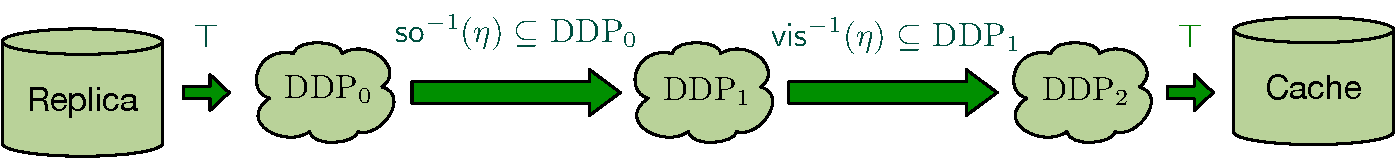
\includegraphics[scale =
	0.4]{Figures/Availability_deg.pdf}
	%}
	\\ 
	\hrulefill
\caption{Example of stepwise progress of effects before entering the
cache}
\label{fig:avail_deg}
\end{figure}

In this part, we will explain the behavioral outline of our algorithm
using an example. The formal operational semantics of this approach can be
found in appendix \ref{appendix:large_semantics}.

Let's assume we are given a contract $\psi=\forall (a,b). a
\xrightarrow{\soZ;\visZ;\soZ}b \Rightarrow a \xrightarrow{\visZ} b$, and
we want replicas to maintain consistent caches according to this
contract. We explain our approach by
explaining a replicas' behavior when certain events occur: 
\begin{itemize}
\item {\bf Remote Effect Arrival:} When a new remote effect arrives to the
replica, it is simply added to the set of local effects and 
its $DDP$ is initially set to 0. Since the length of the
given contract is 3, as we will see shortly the effect requires two
steps
of $DDP$ refreshes, before it can enter the cache.
\item {\bf Operation Submission: } Since the given contract is an LB
type, the replica must now make sure that all effects from ealier
operations of the same session, are present in the \emph{cache} and if
not, 
block the operation temporarily. The operation can proceed and
wtiness \emph{all} effects at the replica, after the mentioned effects enter
the cache.
\item {\bf Cache Refresh: } The replica, must periodically perform 
cache refreshes and move effects from $DDP_2$ to the cache. As explained
we know that the complete set of dependencies for these effects are
already present. 
\item {\bf DDP Refresh: } At this periodic step, $DDP$ of effects are
updated by checking if they can be given a larger one. 
At each step the $DDP$ of an effect $\eff$ is increased from $i$ to $i+1$ if
all effects in $r_{i+1}^{-1}(\eff)$ already have $DDP$ value at least equal to $i$.
In this example, an effect $\eff$ that has the initial $DDP$ value 0, can get
the value 1, only if all effects in  $\soZ^{-1}(\eff)$ are already
present at the replica which means they have $DDP$ value of at least 0.
Similarly, effects that have the $DDP$ value of 1 can get the value 2,
if all effects in their $\visZ^{-1}$ set, have the $DDP$ value of
minimum 1. At this point, effects have reached the value 2, which means
they can be now moved to the cache at the next cache refresh (Figure
\ref{fig:avail_deg}).
\end{itemize}

Note that, in case one of the elements of the given relation is a
closure, for example assume the given relation is $\xrightarrow{so;vis^*;so}$,
we can avoid all recursive computations, by allowing an effect $\eff$
to go from $DDP_1$ to $DDP_2$, only if $vis^{-1}(\eff)$ is present in
$DDP_1$ {\bf and} in $DDP_2$. This way, we are sure that the same
condition was also checked for all effects in $vis^{-1}(\eff)$ before they
entered $DDP_2$, which brings us the desired behavior, without any
computations involving closures.




